%%%%%%%%%%%%%%%%%%%%%%%%%%%%%%%%%%%%%%%%%%%%%%%%%%%%%%%%%%%%%%%%%%%%%%
% CS624: Analysis of Algorithms
% Copyright 2015 Pejman Ghorbanzade <mail@ghorbanzade.com>
% Creative Commons Attribution-ShareAlike 4.0 International License
% More info: https://bitbucket.org/ghorbanzade/umb-cs624-2015s
%%%%%%%%%%%%%%%%%%%%%%%%%%%%%%%%%%%%%%%%%%%%%%%%%%%%%%%%%%%%%%%%%%%%%%

\section*{Question 6}
Let $T$ be a rooted tree. $T$ is not necessarily a binary tree. That is, each node may have any finite number of child. We are going to consider a method of visiting each node of the tree. The method works as follows.

At step 1, we visit the root. The root is then marked as \textit{visited}.
At step $n$, all nodes that have already been marked \textit{visited} can visit at most one of their children. Of course if all the children of a node have already been visited, there is nothing for that node to do. But other nodes may stil do something at that step. So in particular, more than one node might be visited in a single step of the process.

What is the minimum number of steps necessary to visit 
every node in the tree?

\begin{enumerate}[label=(\alph*)]
\item Draw a tree in which more than one node is visited at some step of this process, and show why that happens.

\item Show that this problem contains optimal substructure. State precisely and clearly what the substructure is and show why it is optimal.

\item Use that result to write a recursive algorithm to solve this problem.

\item Turn that algorithm into a dynamic programming algorithm.

\item What is the cost of your proposed algorithm, i.e. what is the cost of the algorithm that computes the cost?
\end{enumerate}

\subsection*{Solution}

\begin{enumerate}[label=(\alph*)]
\item Figure \ref{fig61} shows a tree at step 3 in which more than one node is \textit{visited}.

\begin{figure}[H]\centering
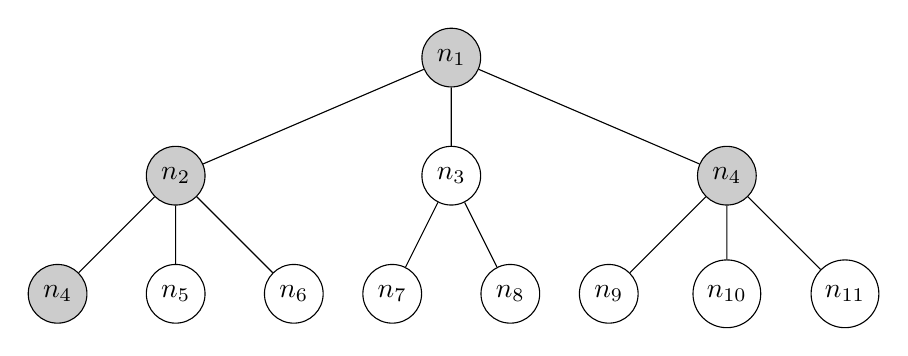
\begin{tikzpicture}[level distance=1.5cm,
  level 1/.style={sibling distance=3.5cm},
  level 2/.style={sibling distance=1.5cm}]
\node[circle,draw,fill=black!20]{$n_1$}
child{
  node[circle,draw,fill=black!20]{$n_2$}
  child{
    node[circle,draw,fill=black!20]{$n_4$}
  }
  child{
    node[circle,draw]{$n_5$}
  }
  child{
    node[circle,draw]{$n_6$}
  }
}
child{
  node[circle,draw]{$n_3$}
  child{
    node[circle,draw]{$n_7$}
  }
  child{
    node[circle,draw]{$n_8$}
  }
}
child{
  node[circle,draw,fill=black!20]{$n_4$}
  child{
    node[circle,draw]{$n_9$}
  }
  child{
    node[circle,draw]{$n_{10}$}
  }
  child{
    node[circle,draw]{$n_{11}$}
  }
};
\end{tikzpicture}
\caption{A sample tree with proposed structure}\label{fig61}
\end{figure}

\end{enumerate}
